\documentclass{article}
\usepackage[T1]{fontenc}
\usepackage[utf8]{inputenc}
\usepackage{amsmath}
\usepackage{amssymb}
\usepackage{hyperref}
\usepackage{parskip} %skip the indent of a new paragraph.
\usepackage{float}
\usepackage{graphicx}
\usepackage{listings}
\usepackage[per-mode=symbol]{siunitx}
\usepackage{epstopdf}
\usepackage[super]{nth}
\lstset{language=Matlab, frame=single, breaklines=true,numbers=left, keywordstyle=\color{blue},rulecolor=\color{black},commentstyle=\color{gray}}

\usepackage{cleveref}
\usepackage{todonotes}

%% Brukes for tabeller (av likninger)
\usepackage{tabularx}
\def\tabularxcolumn#1{m{#1}}

\newcommand{\TODO}[1]{\todo[inline]{#1}}
\newcommand{\mbf}[1]{\mathbf{#1}} % Arg 1 is bold (in math environment)
\newcommand{\partialderiv}[2]{\frac{\partial{#1}}{\partial{#2}}} % prints partial derivative as a fraction

\title{Linear Systems TTK4115 - Boat Lab Report}
\author{Bern Johan Damslora -- 759477 \\ Didrik rokhaug -- 759528}
\date{\today}

\begin{document}

% !TEX root = main.tex

\begin{titlepage}
    %\maketitle
    %\rule{\linewidth}{0.5mm}
    \begin{center}
    	\large
    	Linear Systems TTK4115
    \end{center}
    \vspace{\fill}
    \rule{\linewidth}{0.5mm}
    \begin{center}
    	\huge
    	Boat Lab Report
    \end{center}
	\rule{\linewidth}{0.5mm}
	\vspace{\fill}

	%\begin{center}
    %	\huge
    %	Bern Johan Damslora -- 759477 \\ Didrik rokhaug -- 759528
    %\end{center}
    \large
    \centering
    Group 33:
    \begin{table}[H]
    	\centering
    	\large
    	\begin{tabular}{rl}
    		\textbf{Bernt Johan Damslora} & (nr. 759477) \\
    		\textbf{Didrik Rokhaug} &  (nr. 759528)

    	\end{tabular}
    \end{table}
    \vspace{\fill}
    \begin{center}
    	\large
    	\today
    \end{center}
	\vspace{\fill}
    \begin{figure}[H]
    \centering
    
\includegraphics[width=0.5\textwidth]{images/logontnu_eng}
    \end{figure}
    \thispagestyle{empty}
\end{titlepage}


%\section*{Table of contents}
\tableofcontents
\listoffigures
\thispagestyle{empty} %Avoid page numbering on the table of contents
\newpage

\setcounter{page}{1}
% Part 1
% !TEX root = main.tex
\section{Part 1: Identification of the boat  parameters}

In the assignment text we were given the following model of a ship:
\begin{subequations}
	\label{eq:completeModel}
		\begin{align}
				\dot{\xi_w} &= \phi_w \label{eq:xi_w}\\
				\dot{\phi_w} &= -\omega_0^2\xi_w-2\lambda\omega_0\phi_w+K_ww_w \label{eq:phi_w}\\
				\dot{\phi} &= r \label{eq:phi} \\
				\dot{r} &= -\frac{1}{T}r+\frac{K}{T}(\delta-b) \label{eq:r} \\
				\dot{b} &= w_b \label{eq:b} \\
				y &= \phi + \phi_w + v \label{eq:y}
		\end{align}
\end{subequations}

Where $\phi$ is the average heading, $\phi_w$ is a high frequency component due to the wave disturbance, $r$ the yaw rate and $b$ is a bias to the rudder angle $\delta$, $w_w$ and $w_b$ are white noice disturbances, $v$ is meassurement noise and $K$, $T$, $\lambda$ and $\omega_0$ are model parameters.

Using this model we can find the transfer function from $\delta$ to $\phi$. taking the laplace transform of \cref{eq:phi} and \cref{eq:r} yields
\begin{subequations}
	\begin{align}
		s\phi &= r \label{eq:Lphi}\\
		sr &= -\frac{1}{T}r+\frac{K}{T}(\delta-b) \label{eq:Lr}
	\end{align}
\end{subequations}

Assuming no disturbances $b = 0$ and combining \cref{eq:Lphi} with \cref{eq:Lr} gives
\begin{equation}
	H(s) = \frac{\phi}{\delta}(s) = \frac{K}{s^2T+s}
\end{equation}


% Part 2
% !TEX root = main.tex

\section{Part 2: Identification of wave spectrum model}

\subsection{2a)}

% Si noe om hva oppgaven er (finne \omega_0 og \lambda)

\todo{Vil Bernt Johan skrive dette som har gjort det?}

\subsection{2b)}
To find the values of $\omega_0$ and $\lambda$ we can compare the estimated PSD of the waves with an analytical, found by using the model of the waves. In order to do this we first need to find the transfer function from $w_w$ to $\psi_w$. This can be done by taking the laplace transform of \todo{insert reference} and \todo{insert reference} yielding

\todo[inline]{Insert equations here}


% Part 3
% !TEX root=main.tex

\section{Part 3: Control system design}

\subsection{3a)}

We want to design a limited PD controller with the transfer function

\begin{equation}
    H_{pd}(s) = K_{pd}\frac{1+T_ds}{1+T_fs} \label{eq:H_pd}
\end{equation}

to control the heading $\psi$ of the ship, by setting the rudder angle $\delta$. We want the cross frequency and phase margin of the open loop system to be $0.10\si{\radian\per\second}$ and $50$ degrees respectively. We also want the time constant $T_d$ to equal the time constant of the system. In order to choose $K_{pd}$, $T_d$ and $T_f$ we first find the transfer function of the open loop system

\begin{equation}
    H_{sys}(s) = H_{pd}(s) \cdot H_{ship}(s) = KK_{pd}\frac{1+T_ds}{s(Ts+1)(T_fs+1)} \label{eq:H_sys}
\end{equation}

As we want $T_d$ to equal the time constant of the model we set $T_d = T = 86.5246 \si{\second}$. Next we use that the phase margin of a system is equal to $\angle H(j\omega_c) + 180 \si{\degree}$.

\begin{subequations}
    \begin{align}
        \angle H_{sys}(j\omega_c) + 180 \si{\degree} &= 50 \si{\degree} \\
        \angle \frac{KK_{pd}}{(j\omega_c)^2T_f+j\omega_c} &= -130 \si{\degree}\\
        \angle KK_{pd} - \angle ((j\omega_c)^2T_f+j\omega_c) &= -130 \si{\degree} \\
        \angle ((j\omega_c)^2T_f+j\omega_c) &= -130\si{\degree} \\
        \tan^{-1}\frac{\omega_c}{\omega_c^2T_f} &= 50 \si{\degree} \\
        T_f &= \frac{1}{ \omega_c \tan (50 \si{\degree}) } \\
        T_f &= 8.3910 \si{\second} \label{eq:T_f}
    \end{align}
\end{subequations}

Last we find $K_{pd}$ by using the definition of the cross frequency: $|H(j\omega_c)| = 1$. This yields

\begin{subequations}
    \begin{align}
        |H_{sys}(j\omega_c) &= 1 \\
        |H_{sys}^2(j\omega_c) &= 1^2 \\
        \left | \frac{KK_{pd}}{s^2T_f+s} \right |^2 &= 1 \\
        \frac{(KK_{pd})^2}{(\omega_c^2 T_f)^2 + \omega_c^2} &= 1 \\
        K_{pd} &= \frac{\sqrt{(\omega_c^2 T_f)^2} + \omega_c^2}{K} \label{eq:K_pd(T_f)}
    \end{align}
\end{subequations}

Inserting \cref{eq:T_f} into \cref{eq:K_pd(T_f)} yields a $K_{pd} = 0.7494$. The controller was implemented in Simulink as seen in \cref{fig:pd}.

\begin{figure}
    \centering
    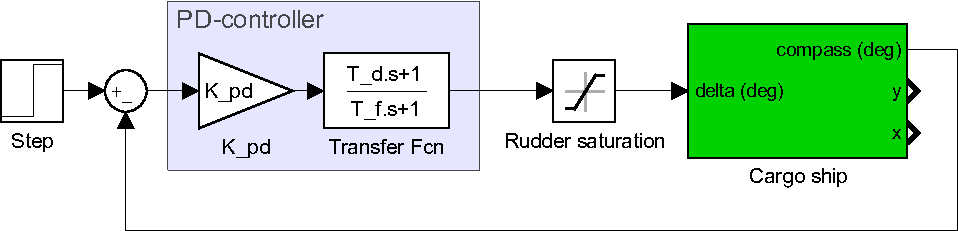
\includegraphics[width=\textwidth]{images/oppg3/a_pd-loop.pdf}
    \caption{Simulink implementation of the PD-controller}
    \label{fig:pd}
\end{figure}

\subsection{3b)}

As we can see in \cref{fig:step_no_dist} the controller does a good job when there are no disturbances. The ship reaches the reference $\psi_r$ of $30\si{\degree}$ within 2 minutes, and the rudder angle is relatively constant over time.

\begin{figure}
    \centering
    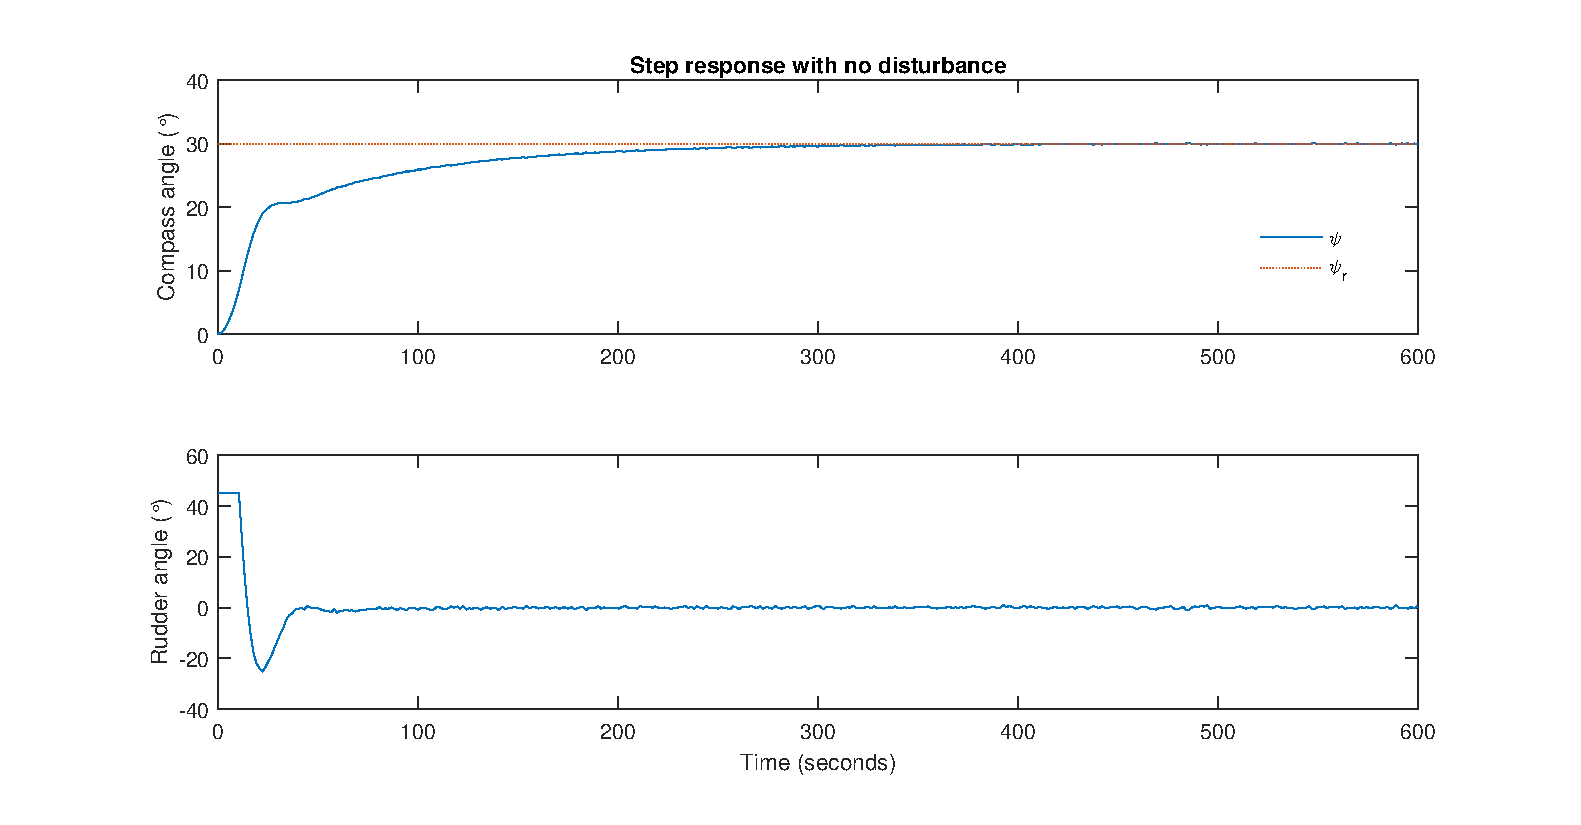
\includegraphics[width=\textwidth]{images/oppg3/stepresp_no_disturbance.eps}
    \caption{Step response of the controller. No disturances.}
    \label{fig:step_no_dist}
\end{figure}

\subsection{3c)}

In \cref{fig:step_current_dist} we see the response of the controller with current disturbance. as we can see the controller is unable to counteract the constant disturbance of the current, which leads to a large constant deviation from the setpoint.

\begin{figure}
    \centering
    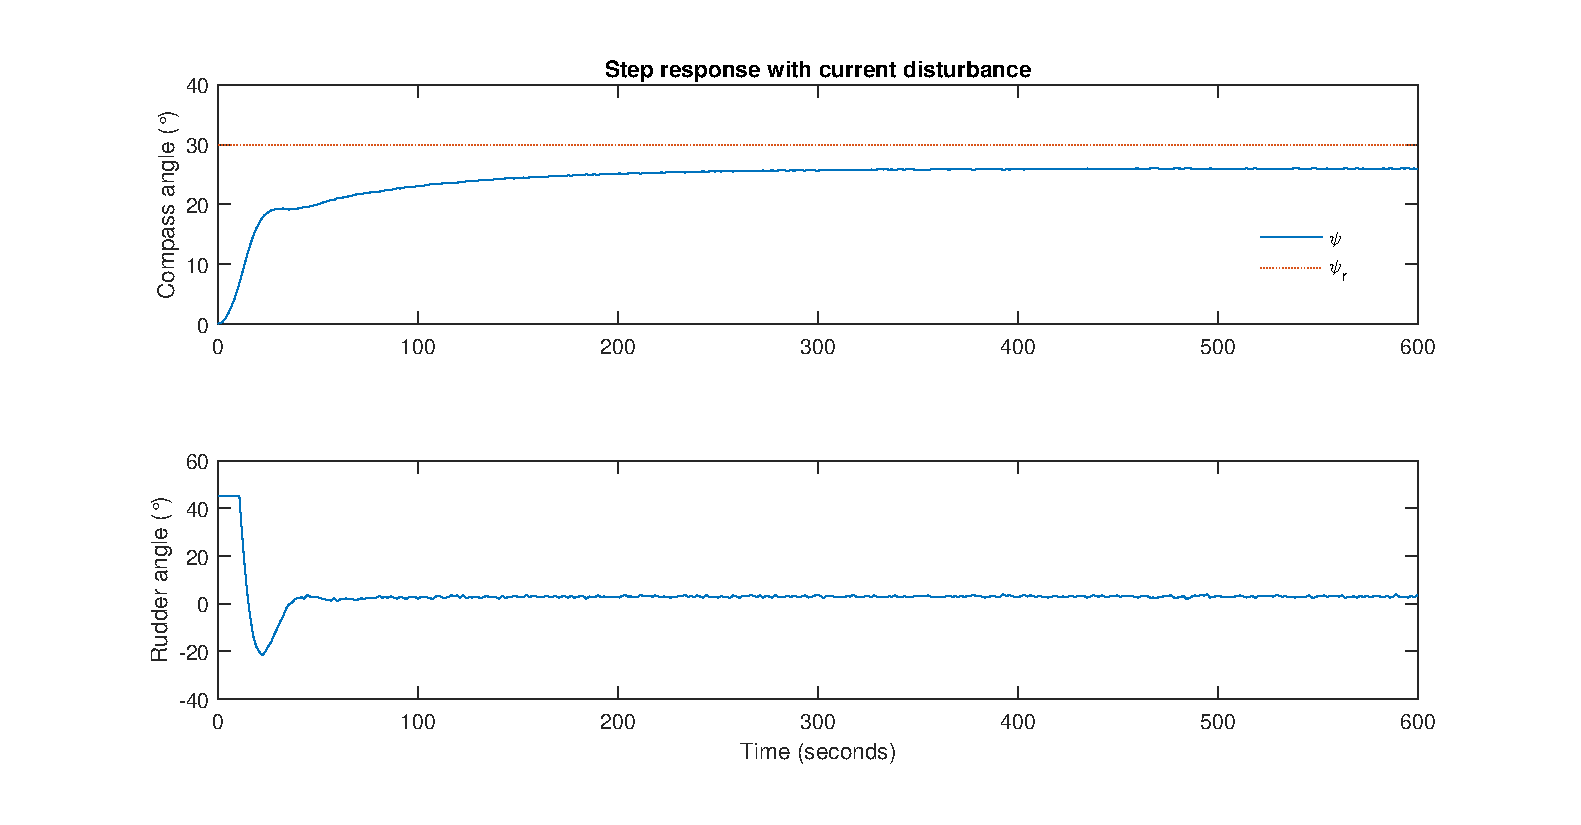
\includegraphics[width=\textwidth]{images/oppg3/stepresp_current_disturbance.eps}
    \caption{Step response of the controller. With current disturbance.}
    \label{fig:step_current_dist}
\end{figure}

\subsection{3d)}

When we apply wave current (and turn off current disturbance), we see that the controller does it best to remove the noise but is unable to do much. In its attempt to remove the noise it applies a lot of rudder input, which if the boat was real would stress the physical system.

\begin{figure}
    \centering
    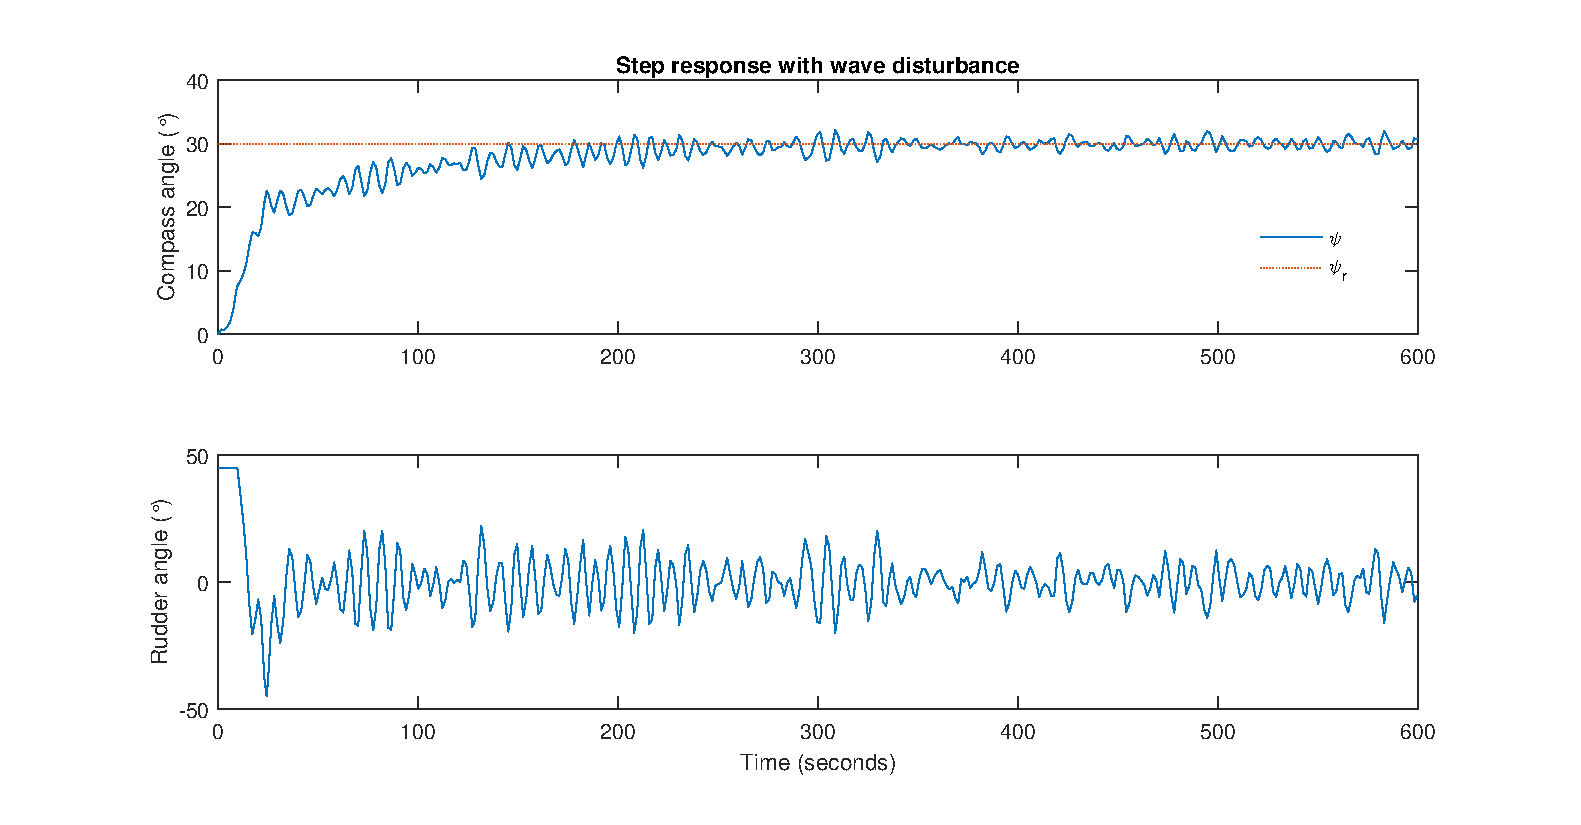
\includegraphics[width=\textwidth]{images/oppg3/stepresp_wave_disturbance.eps}
    \caption{Step response of the controller. With wave disturbance}
    \label{fig:step_wave_dist}
\end{figure}


% Part 4
% !TEX root=main.tex

\section{Observability}

\subsection{Defining the matrices of the model system} \label{subsec:4a}

The model in \cref{eq:completeModel} can be written on the form $\mathbf{\dot x} = \mathbf{A} \mathbf{x} + \mathbf{B}u + \mathbf{E}\mathbf{w}$, $ y = \mathbf{C}\mathbf{x} + v$, with $\mathbf{x} = [ \xi_w\ \psi_w\ \psi\ r\ b]^ T $ , $ u = \delta $ and $ \mathbf{w} = [w_w\ w_b]^T$. Then the matrices $\mathbf{A}$, $\mathbf{B}$, $\mathbf{C}$ and $\mathbf{E}$ are

\begin{subequations}
    \begin{align}
        \mathbf{A} &= \begin{bmatrix}
        0 & 1 & 0 & 0 & 0 \\
        -\omega_0^2 & -2\lambda\omega_0 & 0 & 0 & 0 \\
        0 & 0 & 0 & 1 & 0 \\
        0 & 0 & 0 & -1/T & -K/T \\
        0 & 0 & 0 & 0 & 0
        \end{bmatrix} \\
        \mathbf{B} &= \begin{bmatrix}
        0 \\
        0 \\
        0 \\
        K/T \\
        0 \\
        \end{bmatrix} \\
        \mathbf{E} &= \begin{bmatrix}
        0 & 0 \\
        K_w & 0 \\
        0 & 0 \\
        0 & 0 \\
        0 & 1 \\
        \end{bmatrix} \\
        \mathbf{C} &= \begin{bmatrix}
        0 & 1 & 1 & 0 & 0
        \end{bmatrix}
    \end{align}
\end{subequations}

\subsection{Observability without disturbances} \label{subsec:4b}

 We first checked observability without any disturbance. To do this we removed the disturbances from the system. the resulting $\mathbf{A}$ and $\mathbf{C}$ matrices were

\begin{subequations}
    \begin{align}
        \mathbf{A} &= \begin{bmatrix}
        0 & 1 \\
        0 & -1/T
        \end{bmatrix} \\
        \mathbf{C} &= \begin{bmatrix}
        1 & 0
        \end{bmatrix}
    \end{align}
\end{subequations}

To find out whether the system is observable we checked if \texttt{rank(obsv(A, C)) == size(A,1)}. This code calculates the rank of the observability matrix $\mathcal{O}$, and compares it to the dimension of the matrix $\mathbf{A}$. Using this code we found that the system is observable without any disturbance.

\subsection{Observability with a current disturbance}

Next we checked observability with the current disturbance. The $\mathbf{A}$ and $\mathbf{C}$ matrices used were

\begin{subequations}
    \begin{align}
        \mathbf{A} &= \begin{bmatrix}
        0 & 1 & 0 \\
        0 & -1/T & -K/T \\
        0 & 0 & 0
        \end{bmatrix} \\
        \mathbf{C} &= \begin{bmatrix}
        1 & 0 & 0
        \end{bmatrix}
    \end{align}
\end{subequations}

Using the code in \cref{subsec:4b} we found that the system is observable with current disturbance.

\subsection{Observability with wave disturbance}

Next we checked observability with the wave disturbance. The $\mathbf{A}$ and $\mathbf{C}$ matrices used were

\begin{subequations}
    \begin{align}
        \mathbf{A} &= \begin{bmatrix}
        0 & 1 & 0 & 0 \\
        -\omega^2 & -2\lambda\omega_0 & 0 & 0 \\
        0 & 0 & 0 & 1 \\
        0 & 0 & 0 & - 1/T
        \end{bmatrix} \\
        \mathbf{C} &= \begin{bmatrix}
        0 & 1 & 1 & 0
        \end{bmatrix}
    \end{align}
\end{subequations}

Using the code in \cref{subsec:4b} we found that the system is observable with wave disturbance.

\subsection{Observability with both disturbances}

Next we checked observability with both current and wave disturbance. The $\mathbf{A}$ and $\mathbf{C}$ matrices used were

\begin{subequations}
    \begin{align}
        \mathbf{A} &= \begin{bmatrix}
        0 & 1 & 0 & 0 & 0 \\
        -\omega_0^2 & -2\lambda\omega_0 & 0 & 0 & 0 \\
        0 & 0 & 0 & 1 & 0 \\
        0 & 0 & 0 & -1/T & -K/T \\
        0 & 0 & 0 & 0 & 0
        \end{bmatrix} \\
        \mathbf{C} &= \begin{bmatrix}
        0 & 1 & 1 & 0 & 0
        \end{bmatrix}
    \end{align}
\end{subequations}

Using the code in \cref{subsec:4b} we found that the system is observable with both wave and current disturbance.


% Part 5
% !TEX root=main.tex

\section{Discrete Kalman filter}

\subsection{5a)}

To make a discrete Kalman filter we need to discretize the model found in \cref{subsec:4a}. The discretized system can be found using the equations

\begin{subequations}
    \begin{align}
        A_d &= e^{AT_s} \\
        B_d &= \int_0^{T_s} e^{A\tau}B d\tau \\
        E_d &= \int_0^{T_s} e^{A\tau}E d\tau \\
        C_d &= C
    \end{align}
\end{subequations}

This can be done using he MatLab function \texttt{[Ad, Bd] = c2d(A, B, Ts)} to get the discretized matrices $A_d$ and $B_d$ discretized with a timestep of \texttt{Ts}. To get the model discretized with a sampling frequency of $10\si{\hertz}$ we set \texttt{Ts} to $0.1$. In order to get $E_d$ we use the same function, but swap \texttt{Bd} and \texttt{B} with \texttt{Ed} and \texttt{E}. The resulting $A_d$, $B_d$ and $E_d$ matrices are

\begin{subequations}
    \begin{align}
        A_d &= \begin{bmatrix}
        0.1000 & 0.0993 & 0 & 0 & 0 \\
        -0.0607 & 0.9841 & 0 & 0 & 0 \\
        0 & 0 & 1 & 0.0999 & -1.0063 \cdot 10^{-5} \\
        0 & 0 & 0 & 0.1000 & -0.0002 \\
        0 & 0 & 0 & 0 & 1
        \end{bmatrix} \\
        B_d &= \begin{bmatrix}
        0 \\
        0 \\
        1.0062 \cdot 10^{-5} \\
        0.0002 \\
        0
        \end{bmatrix} \\
        E_ d &= \begin{bmatrix}
        2.4880\cdot 10^{-5} & 0 \\
        0.0005 & 0 \\
        0 & -3.3545\cdot 10^{-7} \\
        0 & -1.0063\cdot 10^{-5} \\
        0 & 0.1000
        \end{bmatrix}
    \end{align}
\end{subequations}


% Osv.

%uncomment to add reference list
%\newpage
%\input{reference}

\end{document}
